\section{ФУНКЦИОНАЛЬНОЕ ПРОЕКТИРОВАНИЕ}
\label{sec:func}

Данный раздел посвящён разработке функциональной схемы, выбору оборудования
разрабатываемой локальной компьютерной сети, её функциональному проектированию и настройке.
Схема функциональная приведена в приложении Б.

\subsection{Обоснование выбора сетевого оборудования}\label{subsec:func:Equipment}

При построении локальной компьютерной сети используется следующее оборудование:
маршрутизатор, коммутатор, беспроводные точки доступа, моноблоки, также принтер и сканеры.
Также, необходимо учесть, что должно приобретаться оборудование фирмы Allied Telesis, поскольку это условие было указано заказчиком.
В следующих подразделах описано обоснование выбора конкретных моделей перечисленного оборудования.

\subsubsection{Обоснование выбора операционной системы}\label{subsubsec:func:OSChoice}

    Так как разрабатываемая локальная компьютерная сеть по требованию заказчика должна быть бюджетной,
    то выбор операционной системы склоняется к операционной системе,
    свободно распространяющейся в сети интернет и не требующей покупки платной лицензии.
    Классическими примерами такой операционной системы являются дистрибьютивы, построенные на ядре Linux.

    Выбор дистрибутива Linux зависит от потребностей конкретного пользователя или организации.
    После проведения анализа плюсов и минусов различных дистрибьютивов первое место занял дистрибьютив Linux Ubuntu.
    Ubuntu имеет ряд характеристик, которые выделяют его на фоне остальных дистрибьютивов:

    \begin{itemize}
        \item Простота установки и использования;
        \item Обширное сообщество поддержки;
        \item Многообразие программного обеспечения;
        \item Легкость в поиске и установке программ;
        \item LTS-версии;
    \end{itemize}

\subsubsection{Обоснование выбора пользовательских станций}\label{subsubsec:func:PCChoice}
    Выбор компьютеров для организации, занимающейся торговлей компьютерными комплектующими,
    не зависит от отделов организации, так как все отделы имеют схожие задачи,
    которые не связаны с высокой вычислительной нагрузкой.
    Например, для отдела продаж, бухгалтерии и учёта не требуется техника, которая должна производить большое количество вычислений.
    Прежде чем приступить к выбору конкретных компонентов, следует выделить состав любой пользовательской станции.

    \begin{itemize}
        \item Процессор;
        \item Оперативная память;
        \item Жесткий диск;
        \item Графическая карта(встроенная либо дискретная);
        \item Сетевые адаптеры;
        \item Безопасность;
        \item Дисплей;
    \end{itemize} \\

    Дополнительно к ПК требуется выбрать следующие комплектующие:

    \begin{itemize}
        \item Компьютерная мышь;
        \item Клавиатура;
    \end{itemize}


    Так как в вышеоговоренных требования к ПК нет пункта высокопроизводительных вычислений, то в качестве реальных решений будут рассмотрены готовые моноблоки.
    Данное решение также выбрано в целях экономии времени на монтажных работах и поиске комплектующих.

    Выбор готовых решений будет производиться на популярном сайте-агрегаторе товаров Onliner.by в которых есть возможность фильтрации товара.
    Так как в пункте 3.1.1 операционнонная система, которая будет установлена на персональные компьютеры, уже была выбрана,
    то при помощи фильтров был произведён поиск бюджетных комплексных решений с целью нахождения ПК с уже предустановленной операционной системой Linux Ubuntu.
    Одним из найденных решений оказался Моноблок SunWind Action AiO 21i.
    SunWind Action AiO 21i выделился на фоне остальных комплексных решений низкой ценой и тем, что в комплектации к моноблоку прилагается клавиатура и компьютерная мышь.
    Моноблок имеет процессор Intel Celeron N4020 2800 МГц, 256 ГБ SSD накопитель и 4 ГБ ОЗУ.

\subsubsection{Обоснование выбора антивируса}\label{subsubsec:func:Antivirus}
Обеспечение безопасности компьютерных сетей включает в себя ряд мероприятий и технологий,
направленных на предотвращение, обнаружение и ответ на вирусные угрозы.
Однако ключевым способом защиты от вирусов является антивирус.
Ubuntu — это дистрибутив Linux, и в отличие от Windows, Linux не так часто подвергается воздействию вирусов и вредоносного ПО.
Однако, пользователи Linux могут использовать антивирусное программное обеспечение.
Вот основные антивирусные программы, которые могут быть использованы на Ubuntu:
\begin{itemize}
    \item ClamAV;
    \item Sophos Anti-Virus for Linux;
    \item ESET NOD32 Antivirus for Linux;
\end{itemize}
Из представленных был выбран ClamAV, так как он является свободным и открытым антивирусом, разработанным специально для систем Linux.
Свободный означает, что для его использования не требуется покупки лицензии и он может быть установлен прямо из командной строки.
Он часто используется для сканирования электронной почты на наличие вредоносных вложений, а также общедоступных директорий.
Это является большим плюсом в обеспечении безопасности для персональных компьютеров работников организации,
занимающейся торговлей компьютерными комплектующими, так как их работа напрямую связана с электронной почтой и для файлового сервера этой организации.

\subsubsection{Обоснование выбора принтера}\label{subsubsec:func:PrinterChoice}
    Для выбора существующих принтеров также воспользуемся сайтом-агрегатором Onliner.by.

    В качестве принтера выбор встал между “HP M203dn” и “Pantum M6550NW”.
    Сравнение характеристик принтеров привидены в таблице 3.1.

    \begin{longtable}{
        | >{\raggedright}m{0.4\textwidth}
        | >{\raggedright}m{0.25\textwidth}
        | >{\raggedright\arraybackslash}m{0.25\textwidth}|}

        \caption{Сравнение характеристик принтеров}
        \label{table:func:printer} \\
        \hline
        \centering
        & \centering\arraybackslash HP M203dn
        & \centering\arraybackslash Pantum M6550NW \\
        \hline
        \endfirsthead

        \caption{продолжение} \\
        \hline
        \centering
        & \centering\arraybackslash HP M203dn
        & \centering\arraybackslash Pantum M6550NW \\
        \hline
        \endhead

        Cкорость печати (страниц в минуту) &
        28 &
        22
        \\ \hline

        Размер картриджа (копий) &
        3500 &
        1600
        \\ \hline

%        Размер картриджа (копий) &
%        3500 &
%        1600
%        \\ \hline

    \end{longtable}

    HP имеет лучшую скорость печати (28 против 22 страниц в минуту), а также значительно больший размер картриджа – до 3500 копий против 1600, за большую стоимость.
    Оба принтера являются лазерными, поэтому этот параметр не учитывался при сравнении.
    Ключевым фактором в пользу Pantum является возможность принтера отправлять сканы изображения на компьютер по сети,
    что может оказаться чрезвычайно полезным, так как работники организации будут находится на нескольких этажах.
    По итогу был выбран принтер “Pantum M6550NW”.

\subsubsection{Обоснование выбора IP-телефона}\label{subsubsec:func:IPPhoneChoice}
    После поиска на торговых площадках в дешевом ценовом сегменте выделился IP-телефон Snom D120.
    Он имеет все необходимые характеристики для очуществления взаимодействия в рамках локальной компьютерной сети,
    а также низкую стоимость по сравнению с конкурентами.
    Также подробная инструкция по настройке этого IP-телефона даёт ещё одну причину для выбора в пользу Snom D120.

\subsubsection{Обоснование выбора файлового сервера}\label{subsubsec:func:ServerChoice}
    При выборе оборудования для NTFS/SMB-сервера также воспользуемся сайтом-агрегатом onliner.by.
    В дешёвом сегменте !!!!!готовых решений файлового сервера были выявлены лишь два устройства компании Synology:
    DiskStation DS115j и DiskStation DS120j.
    Характеристики устройств, учавствовавшие при выборе приведены в таблице 3.2:

    \begin{longtable}{| >{\raggedright}m{0.4\textwidth}
                | >{\centering\arraybackslash}m{0.25\textwidth}
                | >{\centering\arraybackslash}m{0.25\textwidth}|}
    \caption{Сравнение DiskStation DS115j и DiskStation DS120j} \label{table:func:ServerChoice} \\
    \hline
    \arraybackslash
    & \centering\arraybackslash DS115j
    & \centering\arraybackslash DS120j \\
    \hline
%    \endfirsthead % Повторяется на каждой странице
%    \hline
%    \centering\arraybackslash № \\
%    & \centering\arraybackslash Адрес подсети \\
%    & \centering\arraybackslash Длинна маски в битах\\
%    & \centering\arraybackslash Количество хостов\\
%    \hline
    \endhead
    Оперативная память, Мб &
    256 &
    512
    \\
    \hline
    Тип оперативной памяти &
    Нет данных &
    DDR3L
    \\
    \hline
    Интерфейс внутренних накопителей &
    SATA 3.0 &
    SATA 3.0
    \\
    \hline
    Ethernet порты &
    1x 1 Гбит/с &
    1x 1 Гбит/с
    \\
    \hline
    Количество отсеков для накопителей &
    1 &
    1
    \\
    \hline
    \end{longtable}

    При практически одинаковой стоимости страшая модель имеет в два раза больше оперативной памяти,
    поэтому остановимся на ней.

    Также, так как выбранный сервер не имеет встроенного жесткого диска, требуется его выбрать.
    Исходя из количества слотов, нужно выбрать жесткий диск большого размера - от 1 Тб.
    Также для сохранения максимальной скорости чтения и записи интерфейс подключения должет быть SATA 3.0.
    Воспользовавшишь сайтом-агрегатом onliner.by и применив фильтры по параметрам, описанным выше, выбор встал между моделями
    WD Caviar Blue WD10EZEX, Seagate Barracuda ST2000DM008, Seagate Barracuda ST4000DM004.

    \begin{longtable}{| >{\raggedright}m{0.225\textwidth}
                | >{\raggedright\arraybackslash}m{0.220\textwidth}
                | >{\raggedright\arraybackslash}m{0.225\textwidth}
                | >{\raggedright\arraybackslash}m{0.225\textwidth}|}
    \caption{Сравнение жестких дисков} \label{table:func:HDDChoice} \\
    \hline

    & \centering\arraybackslash WD10EZEX
    & \centering\arraybackslash ST2000DM008
    & \centering\arraybackslash ST4000DM004 \\
    \hline
    Тип накопителя
    & HDD
    & HDD
    & HDD \\
    \hline
    Объём
    & 1 ТБ
    & 2 ТБ
    & 4 ТБ \\
    \hline
    Форм-фактор
    & 3.5"
    & 3.5"
    & 3.5" \\
    \hline
    Скорость вращения шпинделя
    & 7200 об/мин
    & 7200 об/мин
    & 5400 об/мин \\
    \hline
    Количество пластин
    & не указано
    & 1
    & 2 \\
    \hline
    Буфер
    & 64 МБ
    & 256 МБ
    & 256 МБ \\
    \hline
    \end{longtable}

    Чем выше плотность записи, тем меньше пластин требуется для обеспечения требуемого объема, и тем выше будет быстродействие (при прочих равных параметрах).
    Более высокая скорость вращения магнитных пластин при прочих равных условиях обеспечивает более высокое быстродействие -
    как при последовательном доступе (данные быстрее поступают в считывающие головки), так и при случайном (меньше времени уходит на ожидание нужного сектора).

    Оптимальным решением для использования внутри файлового сервера является Seagate Barracuda ST2000DM008,
    так как этот жесткий диск имеет наилучшее быстродействие среди представленных в сравнении.

\subsubsection{Обоснование выбора маршрутизатора}\label{subsubsec:func:RouterChoice}
    Основным критерием при выборе маршрутизатора оказалось наличие 2-х Gigabit Ethernet WAN-портов.
    В доступной ценовой категории оказалось два устройства обладающих всеми необходимыми функциями: AR3050S и AR4050S.
    Основные отличия заключаются в мощности процессора, и соответственно пропускной способности файрвола, VPN, IPS и т.д.
    \begin{center}
        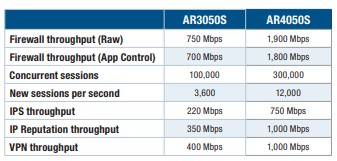
\includegraphics[width=0.7\textwidth]{images/roters}\\
        Рисунок 3.1 – Сравнение пропускной способности
    \end{center}
    \\
    Так как разница в цене составляет лишь 15\% и старшая модель позволит пропускать весь трафик через файрволл было решено остановиться на ней.
    Помимо функции файрволла, данное устройство будет заниматься маршрутизацией в сети, а также между VLAN-ами (поддерживает 802.1Q).

\subsubsection{Обоснование выбора коммутатора}\label{subsubsec:func:SwitchChoice}

    Управляемые коммутаторы дают возможность сконфигурировать каждый порт, а так-же назначить VLAN-ы, что является первым критерием при выборе.
    К управляемому коммутатору будут подключены как минимум 9 других устройств, поэтому вторым критерием будет наличие достаточного кол-ва портов: в общем случае – 16.
    Для уменьшения количества связей данный коммутатор также должен обладать GbE портами.
    Под все вышеперечисленные критерии подошли три линейки коммутаторов: “x230” и “AT-x330-20GTX”, “GS970M”.
    Основные критерии при сравнении приведены в таблице 3.4.

\begin{longtable}{| >{\raggedright}m{0.250\textwidth}
                | >{\raggedright\arraybackslash}m{0.200\textwidth}
                | >{\raggedright\arraybackslash}m{0.250\textwidth}
                | >{\raggedright\arraybackslash}m{0.200\textwidth}|}
    \caption{Сравнение коммутаторов} \label{table:func:switchList} \\
    \hline
    & \centering\arraybackslash AT-x230-18GP
    & \centering\arraybackslash AT-x330-20GTX
    & \centering\arraybackslash AT-GS970M/18 \\
    \hline
    \endfirsthead % Повторяется на каждой странице
    \hline
    & \centering\arraybackslash AT-x230-18GP
    & \centering\arraybackslash AT-x330-20GTX
    & \centering\arraybackslash AT-GS970M/18 \\
    \hline
    \endhead
    Тип & L2+ & L3 & L3 lite \\
    \hline
    Цена & & & Лучшая \\
    \hline
    Порты &
    16 x 1000T, \newline 1 x 1000X SFP &
    16 x 1000T, \newline 2 x 10G-T, \newline 2 x SFP+ &
    16 x 1000T, \newline 2 x 1000X SFP \\
    \hline
    Настраиваемые VLAN & + & + & + \\
    \hline
    Агрегация каналов & + & + & + \\
    \hline
\end{longtable}



    Все приведенные модели обладают необходимым функционалом.
    “x230” и “x330” также, в отличие от “GS970M” поддерживают динамическую маршрутизацию, однако для этих целей было решено использовать маршрутизатор.
    Исходя из всего вышесказанного была выбрана линейка “GS970M”.
    Данная модель также имеет конфигурацию с 24-мя GbE портами.
    Однако в рамках разрабатываемой сети будет достаточно модели “AT-GS970M/18-50”, имеющей 16 портов.

\subsubsection{Обоснование выбора точки беспроводного доступа}\label{subsubsec:func:WirelessPointChoice}

    Также следует определить и количество точек доступа которые могут покрыть этаж вытянутой прямоугольной формы с соотношением сторон 1:4
    с площадью 210 квадратных метров.
    В бюджетной ценовой категории было найдено две подходящих точки доступа: “TQm 1402” и “TQ5403m”.
    Точки доступа на нулевом и первом этажах должны будут работать на два помещения каждая.
    Исходя из этого одним из основных критериев для точки доступа является мощность в диапазоне 2.4 GHz.
    Сравнение мощностей приведено в таблице 3.5.

    \begin{table}[ht]
        \caption{Сравнение мощностей точек доступа}
        \label{table:func:wirelessProperty}
        \begin{tabular}{| >{\raggedright}m{0.310\textwidth}
                        | >{\raggedright\arraybackslash}m{0.310\textwidth}
                        | >{\raggedright\arraybackslash}m{0.310\textwidth}|}
            \hline
            \centering  & \centering\arraybackslash TQm 1402 & \centering\arraybackslash TQ5403m \\

            \hline
            Max. peak gain 2.4 GHz &
            1.9 dBi &
            3.95dBi \\
            \hline
            Max. peak gain 5 GHz &
            3.7 dBi &
            4.20dBi \\
            \hline
        \end{tabular}
    \end{table}

    Питание точки доступа “TQm 1402” осуществляется только через PoE, в то время как для “TQ5403m” предусмотрена возможность питания через адаптер питания.
    Для использования PoE нужен коммутатор со специальным портом, однако это значительно увеличит его стоимость.
    Другим вариантом является использование PoE адаптера, однако стоимость таких адаптеров у Allied Telesis соразмерна стоимости точек доступа.
    Для бюджетной сети предпочтительными вариантами будут:
    \begin{itemize}
        \item использование адаптеров от других производителей (например Адаптер TP-Link “TL-PoE2412G”);
        \item использование обычного адаптера питания при наличии такой возможности.
    \end{itemize}

    Учитывая во внимание все вышеуказанные факторы была выбрана точка доступа “TQ5403m”.
    При наличии электрических розеток рядом с местом ее расположения будет использоваться обычный адаптер питания.
    При отсутствии таковых будет использоваться PoE адаптер TP-Link “TL-PoE2412G”

%--------------------------------------------------------------------------------------

\subsection{Обоснование выбора пассивного сетевого оборудования}\label{subsec:func:passiveEquipment}
Пассивным сетевым оборудованием называется сетевое оборудование, не питающееся от электрической сети, не преобразующее сигнал и выполняющее функции по его усилению.
Примерами такого оборудования можно представить различные кабели, информационные розетки, монтажные шкафы, монтажные стойки, телекоммуникационные шкафы, и многое другое.

    \subsubsection{Выбор сетевого шкафа}
    Для обеспечения удобства организации оборудования и его физической защиты был выбран телекоммуникационный шкаф ШТВ-Н-9.6.5-4ААА.
    Высота составляет 9 U, чего хватит для установки оборудования и разводки кабелей, также останется место для масштабирования сети.
    Корпус обладает защитой от наружного механического удара степени IK 10, внутри покрыт термоизоляционным материалом,
    что и повлияло на его выбор, так как по требованию заказчика должна быть обеспечена повышенная пожарная безопасность.

    \subsubsection{Выбор кабеля}\label{subsubsec:func:WireChoice}

    Часть оборудования будет работать со скоростью до 1Гбит/с, в связи с чем была выбрана витая пара категории 5e.
    Для нее характерны стандарты 10/100/1000BASE-T и дальность до 100 м при использовании 1000BASE-T.
    Помимо этого по требованию заказчика требуется повышенная пожарная безопасность на объекте,
    вследствие чего был выбран кабель U/UTP REXANT CAT 5e ZH нг(А)-HF 4PR 24AWG.
    Маркировка ZH нг(А)-HF указывает на отсутствие галогенов в оболочке кабеля и на то,
    что материалы из которых сделана оболочка плохо поддаются горению.
    Также с такой оболочкой уменьшается эмиссия токсичных газов и дыма в случае пожара.

    \subsubsection{Выбор коннектора, короба и розетки}\label{subsubsec:func:OtherPassiveChoice}
В характеристиках кабеля указан диаметр проводника – 24AWG,
поэтому для расчета размера короба возьмем максимальный диаметр кабеля как 6мм.
В большинстве мест нам нужно проложить либо 2, либо 4-6 кабелей, поэтому возьмем короба размерами 25x16 идущие от шкафа и между этажами и 15x10 идущие непосредственно к розеткам.
Возьмем короба Leiden ELECTRIC 15x10 и Leiden ELECTRIC 25x16.
ПВХ эффективно изолирует проводники, предотвращая короткое замыкание,
а также обеспечивают физическую защиту кабелей.
Также возьмем коннекторы Geplink GL4701 RJ45 и розетки PST00 39047.

\subsection{Адресное пространство}\label{subsec:func:addresses}

Основными требованиями заказчика в проектировании адресного пространства локальной компьютерной сети являются:
внешний статический IPv4-адрес,
внутренняя IPv4-адресация должна использовать публичную подсети,
IPv6-адресация должна обеспечивать взаимодействие в рамках внутренней сети.

Согласно варианту, существует выбор из десяти подсетей.
Подсети в нотации Classless Inter-Domain Routing (далее – CIDR) и количество
доступных адресов для конечных устройств приведены в таблице ниже:

\begin{longtable}{| >{\centering}m{0.03\textwidth}
                | >{\raggedright\arraybackslash}m{0.250\textwidth}
                | >{\centering\arraybackslash}m{0.35\textwidth}
                | >{\centering\arraybackslash}m{0.250\textwidth}|}
    \caption{Предлагаемые подсети в нотации CIDR} \label{table:func:Subnetworks} \\
    \hline
    \arraybackslash №
    & \centering\arraybackslash Адрес подсети
    & \centering\arraybackslash Длинна маски в битах
    & \centering\arraybackslash Количество хостов \\
    \hline
%    \endfirsthead % Повторяется на каждой странице
%    \hline
%    \centering\arraybackslash № \\
%    & \centering\arraybackslash Адрес подсети \\
%    & \centering\arraybackslash Длинна маски в битах\\
%    & \centering\arraybackslash Количество хостов\\
%    \hline
    \endhead
    1 &
    27.101.192.0 &
    18 &
    16382
    \\
    \hline
    2 &
    59.206.0.0 &
    15 &
    262142
    \\
    \hline
    3 &
    79.108.212.0 &
    22 &
    1022
    \\
    \hline
    4 &
    125.112.56.0 &
    21 &
    2046
    \\
    \hline
    5 &
    138.233.64.0 &
    18 &
    16382
    \\
    \hline
    6 &
    145.242.117.56 &
    29 &
    6
    \\
    \hline
    7 &
    165.177.192.0 &
    19 &
    8190
    \\
    \hline
    8 &
    187.214.64.0 &
    19 &
    8190
    \\
    \hline
    9 &
    193.176.127.64 &
    26 &
    62
    \\
    \hline
    10 &
    204.53.168.240 &
    29 &
    6
    \\
    \hline
\end{longtable}

Локальная компьютерная сеть предусматривает следующее количество устройств:
\begin{itemize}
    \item маршрутизатор — 1;
    \item коммутатор — 2;
    \item точка доступа — 2;
    \item принтер — 1;
    \item IP-телефон — 6;
    \item стационарные подключения — 10;
    \item мобильные подключения — 20.
\end{itemize}

Общее количество устройств, не учитывая беспроводные устройства посетителей равно 42.
Также при выборе подсети следует учесть, что в будущем сеть может быть расширена,
поэтому не стоит выбирать сеть со слишком малым адресным пространством,
как и сеть с избыточно большим адресным пространством ввиду его ненадобности.

    \subsubsection{Внешняя IPv4 адресация}\label{subsubsec:func:OutererV4}
    В нашем случае внешний IPv4-адрес, который назначается провайдером статический.
    Для демонстрации настройки оборудования данной локальной компьютерной сети был выбран адрес 27.101.192.1/18,
    так как это первый из подходящих адресов.
    Позже, при реальном воссоздании данной сети, адрес следует заменить на действительно выданный провайдером.

    \subsubsection{Внутренняя IPv4 адресация}\label{subsubsec:func:InnerV4}
    Для внутренней IPv4 адресации нужно использовать публичную подсеть, для этого определим, какие подсети принято считать приватными.
    Под приватными подсетями принято считать:
    \begin{itemize}
        \item 10.0.0.0/8 (то есть всё что начинается на 10.);
        \item 172.16.0.0/12 (с 172.16.0.0 по 172.31.255.255 включительно);
        \item 192.168.0.0/16 (с 192.168.0.0 по 192.168.255.255 включительно).
    \end{itemize}

    Для внутренней адресации IPv4 стоит выбрать подсеть не входящую в эти диапазоны.
    Подсети с номерами 6 и 10 из таблицы ниже имеют недостаточночное количество хостов.
    Подсеть с номером 9 из таблицы ниже не может быть разбита на подсети с достаточным количеством хостов.
    Исходя из этого была выбрана подсеть 79.108.212.0, в рамках которой предусмотрено 1022 хостов.
    Данная подсеть не входит в диапазоны приватных подсетей.
    Эта подсеть будет полностью покрывать все необходимые проводные и беспроводные подключения,
    а также имеет запас адресов для будущего расширения сети.
    Исходя из ролей пользователей, которые имеют доступ к оборудованию, следует разделить подсеть на 6 подсетей.

    \begin{itemize}
        \item Пользовательская (пользовательские ПК, принтеры);
        \item Беспроводная (точка доступа и беспроводные устройства);
        \item Беспроводная гостевая (для беспроводных устройств посетителей организации);
        \item Голосовой (для IP-телефонов);
        \item Файлового сервера (для NTFS/SMB-сервера);
        \item Административная (активное сетевое оборудование).
    \end{itemize}

Схема внутренней адресации IPv4 представлена в таблице 3.7.

\begin{longtable}{| >{\raggedright}m{0.25\textwidth}
                | >{\centering\arraybackslash}m{0.15\textwidth}
                | >{\centering\arraybackslash}m{0.15\textwidth}
                | >{\centering\arraybackslash}m{0.35\textwidth}|}
    \caption{Используемые подсети для внутренней адресации IPv4} \label{table:func:VLANNetworks} \\
    \hline
    \arraybackslash Адрес
    & \centering\arraybackslash Префикс маски
    & \centering\arraybackslash Количество хостов
    & \centering\arraybackslash Назначение сети\\
    \hline
%    \endfirsthead % Повторяется на каждой странице
%    \hline
%    \centering\arraybackslash № \\
%    & \centering\arraybackslash Адрес подсети \\
%    & \centering\arraybackslash Длинна маски в битах\\
%    & \centering\arraybackslash Количество хостов\\
%    \hline
    \endhead
    79.108.212.0 &
    27 &
    30 &
    Пользовательский VLAN (10)
    \\
    \hline
    79.108.212.32 &
    27 &
    30 &
    Беспроводной VLAN (20)
    \\
    \hline
    79.108.212.64 &
    27 &
    30 &
    Беспроводной гостевой VLAN (30)
    \\
    \hline
    79.108.212.96 &
    29 &
    6 &
    VLAN файлового сервера (40)
    \\
    \hline
    79.108.212.168 &
    28 &
    14 &
    Голосовой VLAN (50)
    \\
    \hline
    79.108.212.104 &
    26 &
    62 &
    Административный VLAN (101)
    \\
    \hline
    \end{longtable}

Сетевому оборудованию, относящемуся к административному VLAN, необходимо назначить статические IPv4 адреса.
К административному VLAN также будет относиться административная станция ADMIN-PC.
Информация о назначенных оборудованию адресах приведена в таблице ниже, все приведенные
адреса имеют маску подсети административного VLAN (255.255.255.192).

\begin{longtable}{| >{\raggedright}m{0.2\textwidth}
                | >{\centering\arraybackslash}m{0.40\textwidth}
                | >{\centering\arraybackslash}m{0.30\textwidth}|}
    \caption{Адреса устройств административного VLAN} \label{table:func:AdminVLAN} \\
    \hline
    \centering\arraybackslash Обозначение устройства
    & \centering\arraybackslash Тип устройства
    & \centering\arraybackslash Адрес\\
    \hline
%    \endfirsthead % Повторяется на каждой странице
%    \hline
%    \centering\arraybackslash № \\
%    & \centering\arraybackslash Адрес подсети \\
%    & \centering\arraybackslash Длинна маски в битах\\
%    & \centering\arraybackslash Количество хостов\\
%    \hline
    \endhead
    R0 &
    Маршрутизатор &
    79.108.212.105
    \\
    \hline
    S0 &
    Коммутатор &
    79.108.212.106
    \\
    \hline
    S1 &
    Коммутатор &
    79.108.212.107
    \\
    \hline
    ADMIN-PC &
    Административная станция &
    79.108.212.108
    \\
    \hline
    \end{longtable}

    \subsubsection{IPv6 адресация}\label{subsubsec:func:V6}
    Согласно требованиям заказчика, адресация IPv6 в ЛКС должна обеспечивать взаимодействие в рамках внутренней сети,
    что означает, что необходимо использовать IPv6 Unique-Local Unicast адреса.
    Часть Unique-Local Unicast адреса Global ID необходимо выбрать из диапазона допустимых Global ID.
    Функционального различия в том, какой именно Global ID будет использоваться для адресации сети нет,
    поэтому стоит выбрать такой Global ID, который упростит администрирование сети.
    Был выбран Global ID fd00:1111:2222.
    Такой Global ID будет иметь адрес каждой подсети.
    Часть Unique-Local Unicast Subnet ID должна быть уникальным для каждой подсети 16-битным шестнадцатеричным числом.
    Каждой подсети стоит присвоить Subnet ID, соответствующий номеру VLAN, для упрощения администрирования.
    Адреса IPv6, назначенные подсетям, приведены в таблице ниже.
    Все адреса подсетей имеют префикс длиной 64 бита.

    \begin{longtable}{| >{\raggedright}m{0.45\textwidth}
                | >{\centering\arraybackslash}m{0.45\textwidth}|}
    \caption{Используемые подсети для внутренней адресации IPv6} \label{table:func:V6VLAN} \\
    \hline
    \centering\arraybackslash Адрес
    & \centering\arraybackslash Назначение сети \\
    \hline
%    \endfirsthead % Повторяется на каждой странице
%    \hline
%    \centering\arraybackslash № \\
%    & \centering\arraybackslash Адрес подсети \\
%    & \centering\arraybackslash Длинна маски в битах\\
%    & \centering\arraybackslash Количество хостов\\
%    \hline
    \endhead
    fd00:1111:2222:10::/64 &
    Пользовательский VLAN (10)
    \\
    \hline
    fd00:1111:2222:20::/64 &
    Беспроводной VLAN (20)
    \\
    \hline
    fd00:1111:2222:30::/64 &
    Беспроводной гостевой VLAN (30)
    \\
    \hline
    fd00:1111:2222:40::/64 &
    VLAN файлового сервера (40)
    \\
    \hline
    fd00:1111:2222:50::/64 &
    Голосовой VLAN (50)
    \\
    \hline
    fd00:1111:2222:101::/64 &
    Административный VLAN (100)
    \\
    \hline
    \end{longtable}


    Сетевому оборудованию, относящемуся к административному VLAN, необходимо назначить статические IPv6 адреса.
    Информация о назначенных оборудованию адресах приведена в таблице ниже, все приведенные адреса имеют маску длиной 64 бита.
    \begin{longtable}{| >{\raggedright}m{0.2\textwidth}
                | >{\centering\arraybackslash}m{0.35\textwidth}
                | >{\centering\arraybackslash}m{0.35\textwidth}|}
    \caption{Адреса устройств административного VLAN} \label{table:func:AdminV6VLAN} \\
    \hline
    \centering\arraybackslash Обозначение
    & \centering\arraybackslash Тип устройства
    & \centering\arraybackslash Адрес\\
    \hline
%    \endfirsthead % Повторяется на каждой странице
%    \hline
%    \centering\arraybackslash № \\
%    & \centering\arraybackslash Адрес подсети \\
%    & \centering\arraybackslash Длинна маски в битах\\
%    & \centering\arraybackslash Количество хостов\\
%    \hline
    \endhead
    R0 &
    Маршрутизатор &
    fd00:1111:2222:101::1000
    \\
    \hline
    S0 &
    Коммутатор &
    fd00:1111:2222:101::1001
    \\
    \hline
    S1 &
    Коммутатор &
    fd00:1111:2222:101::1002
    \\
    \hline
    PC &
    Административная станция &
    fd00:1111:2222:101::1003
    \\
    \hline
    \end{longtable}

%----------------------------------------------Ы

\subsection{Конфигурация сетевого оборудования}\label{subsec:func:DevicesConfig}

%    \subsubsection{Настройка маршрутизатора}
%    Для начала нужно подключиться к CLI маршрутизатора.
%    С помощью кабеля идущего в комплекте подключить маршрутизатор к компьютеру через консольный порт.
%    Расположение порта указано на рисунке как Console port.
%
%    \centering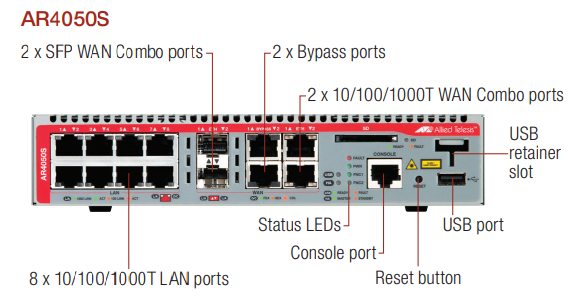
\includegraphics{images/router_config}\label{image:func:RouterPorts} %[width=0.5\textwidth]
%    \centering Рисунок 228 – Расположение портов на AR4050
%
%    Далее с помощью любого клиентского приложения, поддерживающего работу через последовательный порт, например PuTTY начнем работу с маршрутизатором.
%    При настройке других сетевых устройств, в частности точек доступа будем по возможности использовать протокол AMF, который позволяет обнаружить и настроить устройства в сети.
%    Сразу после подключения включим маршрутизатор, зададим имена ему и сети и сделаем его мастером в сети:
%    \begin{verbatim}
%        Awplus>enable
%        Awplus#conf terminal
%        Awplus(config)#hostname Router
%        Router(config)#atmf network-name company
%        Router(config)#atmf master
%    \end{verbatim}
%
%    Также создадим агрегированный канал через который будет проходить соединение с коммутатором на 0 этаже.
%    \begin{verbatim}
%        Router(config)#interface port1.0.0
%        Router(config-if)#channel-group 2 mode active
%        Router(config-if)#exit
%        Router(config)#interface port1.0.1
%        Router(config-if)#channel-group 2 mode active
%        Router(config-if)#exit
%    \end{verbatim}
%
%    Дальнейшие настройки будут производиться через интерфейс с названием “po2”.
%    Занесем в сеть коммутатор подключенный через данный интерфейс:
%    \begin{verbatim}
%    Router(config)#interface po2
%    Router(config-if)#switchport atmf-link
%    \end{verbatim}
%
%    Далее создадим VLAN-ы.
%    Создание административного VLAN-а:
%    \begin{verbatim}
%        Router (config)#vlan database
%        Router (config-vlan)#vlan 4 name vlan4 enable
%        Router (config-vlan)#exit
%        Router (config)#int vlan4
%        Router (config-if)#ip address 192.168.4.0/24
%    \end{verbatim}
%
%    Настроим маршрутизацию между сетями.
%    Для этого для настроим подинтерфейсы для каждого VLAN-а из таблицы 3.9.1. На примере административного VLAN-а пропишем команды:
%    \begin{verbatim}
%        Router (config)#int po2.4
%        Router (config-if)# encapsulation dot1q 4
%        Router (config-if)# ip address 192.168.4.1/24
%    \end{verbatim}
%
%    Далее настроим RIP. Добавим все подсети:
%    \begin{verbatim}
%        Router (config)#router rip
%        Router (config-router)# network 25.237.242.32/28
%        Router (config-router)# network 25.237.160.32/27
%        Router (config-router)# network 25.237.128.32/27
%    \end{verbatim}
%
%%--------------------------------------------------------------------------------

    \subsubsection{Присвоение имен хоста на сетевом оборудовании}
    Перед тем, как приступить к конфигурированию сетевого оборудования,
    каждому устройству стоит присвоить имя хоста, соответствующее его обозначению, приведенному в таблице ниже.
    Для этого необходимо использовать команду hostname.
    Пример настройки имени хоста на маршрутизаторе (R0):
\begin{lstlisting}
awplus(config)#hostname R0
\end{lstlisting}

    \subsubsection{Добавление VLAN}
    На маршрутизаторе и каждом коммутаторе необходимо создать каждый определённый в таблице 3.7 VLAN.
    Пример создания необходимых VLAN на маршрутизаторе R0 [2]:
\begin{lstlisting}
RO(config)#vlan database
RO(config-vlan)#vlan 10,20,30,40,50,101 state enable
\end{lstlisting}

    \subsubsection{Настройка адресации на сетевом оборудовании}
    На коммутаторах необходимо создать виртуальный интерфейс, соответствующий административному VLAN,
    и назначить этому интерфейсу соответствующие IPv4 и IPv6 адреса из таблиц 3.8 и 3.10 соответственно.
    Пример настройки адресации на коммутаторе нулевого этажа (S0) [3]:
\begin{lstlisting}
S0(config)#interface Vlan101
S0(config-if)#ip address 79.108.212.106/26
S0(config-if)#ipv6 enable
S0(config-if)#ipv6 address fd00:1111:2222:101::1001/64
\end{lstlisting}

    На маршрутизаторе на примере VLAN 101 сконфигурируем подинтерфейс:
\begin{lstlisting}
R0(config)#interface port1.0.2
R0(config-if)#encapsulation dot1q 101
R0(config-if)#interface port1.0.2.101
R0(config-if)#ip address 79.108.212.105/26
R0(config-if)#ipv6 enable
R0(config-if)#ipv6 address fd00:1111:2222:101::1000/64
\end{lstlisting}
    Аналогичные действия нужно произвести для каждого VLAN.

    \subsubsection{Реализация удаленного доступа к сетевому оборудованию}
    Для того, чтобы сетевым оборудованием можно было управлять удаленно с административной станции,
    на каждом сетевом устройстве необходимо настроить Secure Shell (SSH).
    Каждому устройству необходимо назначить имя пользователя и пароль,
    которые будут использоваться при подключении административной станции к этому устройству.
    Пример настройки SSH на маршрутизаторе (R0) [4]:
\begin{lstlisting}
S0(config)#crypto key generate hostkey rsa
S0(config)#service ssh
S0(config)#username S0 privilege 1 password z2g2hjh8p
\end{lstlisting}
    Имя пользователя для каждой станции стоит взять такое же, как и имя хоста, для упрощения администрирования.
    Пароль для каждой станции стоит брать произвольный, желательно случайно сгенерированный,
    чтобы обеспечить максимальную безопасность сети.

    \subsubsection{Настройка DHCP и DHCPv6}
    Для того, чтобы не было необходимости назначать каждой пользовательской станции и точке доступа статические адреса IPv4 и IPv6,
    стоит настроить DHCP и DHCPv6 на маршрутизаторе.
    Стоит учесть, что в каждой области DHCP необходимо из набора допустимых адресов исключить адреса,
    которые в будущем будут статически назначены виртуальным интерфейсам коммутаторов и подинтерфейсам маршрутизатора.
    DHCP и DHCPv6 будут настроены для всех VLAN кроме административного и файлового сервера,
    так как адреса административного VLAN назначены на оборудовании статически,
    а адрес для файлового сервера мы назначим вручную при его настройке.
    Пример настройки DHCP и DHCPv6 для пользовательского VLAN (10) [5]:
\begin{lstlisting}[xleftmargin=1]
R0(config)#ip dhcp pool vlan10_dhcp_pool
R0(dhcp-config)#network 79.108.212.0 255.255.255.224
R0(dhcp-config)#range 79.108.212.2 79.108.212.30
R0(dhcp-config)#default-router 79.108.212.1
R0(dhcp-config)#dns-server 8.8.8.8
R0(dhcp-config)#exit
R0(config)#service dhcp-server
R0(config)#ipv6 dhcp pool vlan10_dhcp6_pool
R0(dhcp6-config)#address range fd00:1111:2222:10::2 fd00:1111:2222:10::100
R0(dhcp6-config)#exit
R0(config)#service dhcp6-server
\end{lstlisting}

    Для беспроводного, беспроводного пользовательского и голосового VLAN,
    DHCP и DHCPv6 настраиваются аналогично.

    \subsubsection{Настройка интерфейсов маршрутизатора}
    На маршрутизаторе уже включена функция "ip routing", поэтому необходимо лишь выставить маршрут по умолчанию в Internet:
\begin{lstlisting}
R0(config)#ip route 0.0.0.0/0 27.101.192.1
\end{lstlisting}

    \subsubsection{Настройка интерфейсов коммутаторов}
    Планируется подключить беспроводные точки к следующим двум интерфейсам коммутатора нулевого этажа:
    GigabitEthernet0/8 - GigabitEthernet0/9.
    Для этого на каждом таком интерфейсе необходима конфигурация switchport access.
    Пример конфигурации switchport access для коммутатора нулевого этажа(S0):
\begin{lstlisting}
S0(config)#interface port1.0.2-port1.0.3
S0(config-if)#switchport mode access
S0(config-if)#switchport access vlan 30
S0(config-if)#no shutdown
\end{lstlisting}

Персональные компьютеры и принтер планируется подключить к интерфейсам с
GigabitEthernet 0/8 по GigabitEthernet 0/15 для коммутатора первого этажа
и с GigabitEthernet 0/5 по GigabitEthernet 0/7 для коммутатора нулевого этажа.
Пример конфигурации switchport access для коммутатора нулевого этажа(S0):
\begin{lstlisting}
S0(config)#interface port1.0.5–port1.0.7
S0(config-if)#switchport mode access
S0(config-if)#switchport access vlan 10
S0(config-if)#no shutdown
\end{lstlisting}

Аналогично интерфейсам, к которым подключены беспроводные точки доступа и ПК,
портам, к которым подключены IP-телефоны и файловый сервер, также необходима конфигурация switchport access.

После настроек, приведённых выше, необходимо настроить switchport access для интерфейса,
к которому подключена административная станция (ADMIN-PC).
Для этого используется следующая конфигурация:
\begin{lstlisting}
S1(config)#interface port1.0.3
S1(config-if)#switchport access vlan 101
\end{lstlisting}
В сети предполагается наличие лишь одной административной станции,
поэтому аналогичная настройка на других коммутаторах или интерфейсах не требуется.

    \subsubsection{Настройка беспроводных точек доступа}
    Чтобы настроить беспроводную точку доступа, необходимо подключиться к ее web-интерфейсу.
    Во время процесса настройки, после внесения необходимых изменений на очередной странице интерфейса,
    необходимо их сохранить, нажав кнопку «Save & Apply» в правом нижнем углу страницы
    (в алгоритме действий, приведенном ниже, это действие будет опущено).
    После подключения к web-интерфейсу, необходимо выполнить следующие действия [8]:
    1. Пройти авторизацию, использовав имя пользователя «manager» и пароль «friend».
    2. На странице «Settings > System > Network» задать соответствующее обозначению устройства
    на функциональной схеме имя хоста (см. рисунок ниже).
    \\
    \begin{center}
        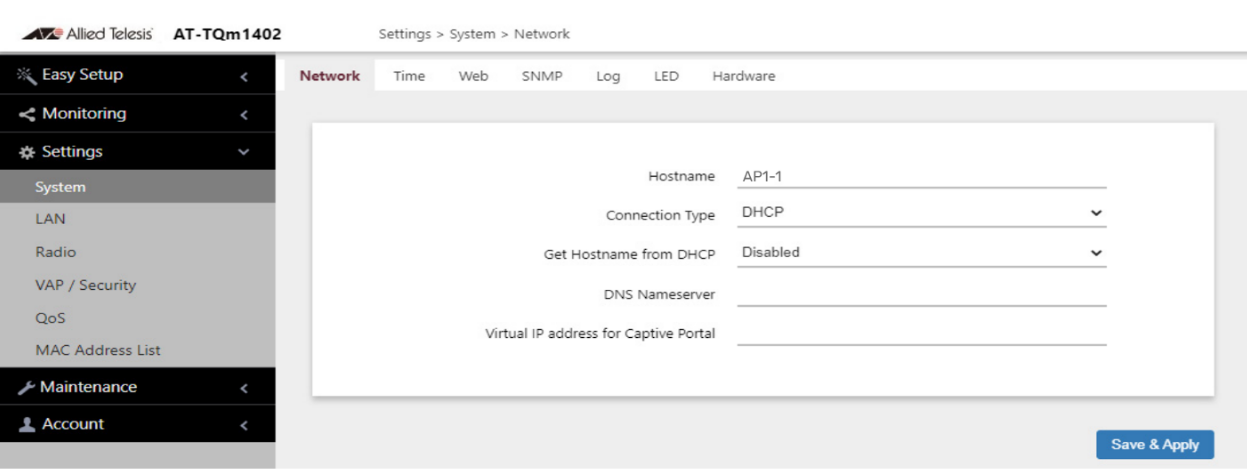
\includegraphics[width=0.9\textwidth]{images/point1}\\
        Рисунок 3.4.1 – Пример изменения имени хоста
    \end{center}
    \\

    3. На странице «Settings > LAN» задать «Management VLAN Tag» «Enabled» и в поле «Management VLAN ID» задать ID «101».
    4. На странице «Settings > VAP / Security > Radio1 > VAP0 > Virtual Access Point»
    задать SSID «Organization» и VLAN ID «20» (см. рисунок 3.5).
    Аналогичные настройки задать и на странице «Settings > VAP / Security >
    Radio2 > VAP0 > Virtual Access Point», но указать SSID «Guests» и VLAN ID «30».

    \\
    \begin{center}
        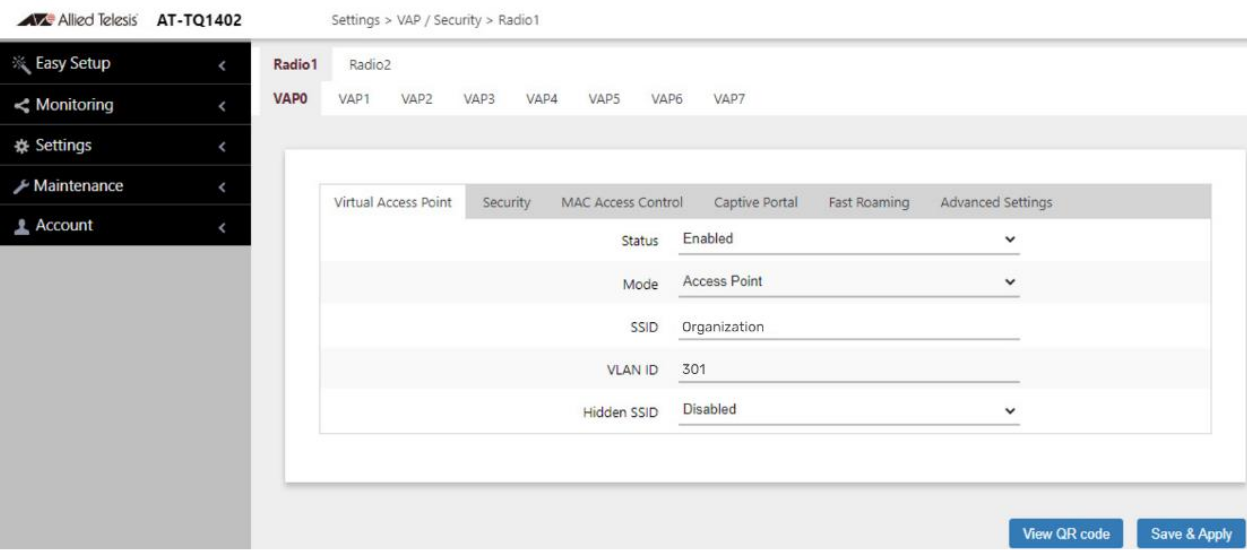
\includegraphics[width=0.9\textwidth]{images/point2}\\
        Рисунок 3.4.2 – Пример настройки Radio1 VAP0
    \end{center}
    \\

    5. На странице «Settings > VAP / Security > Radio1 > VAP0 > Security» выбрать «Mode» «WPA Personal»,
    «WPA Version» «WPA2» и задать пароль в поле «Key» (см. рисунок 3.6).

    \\
    \begin{center}
        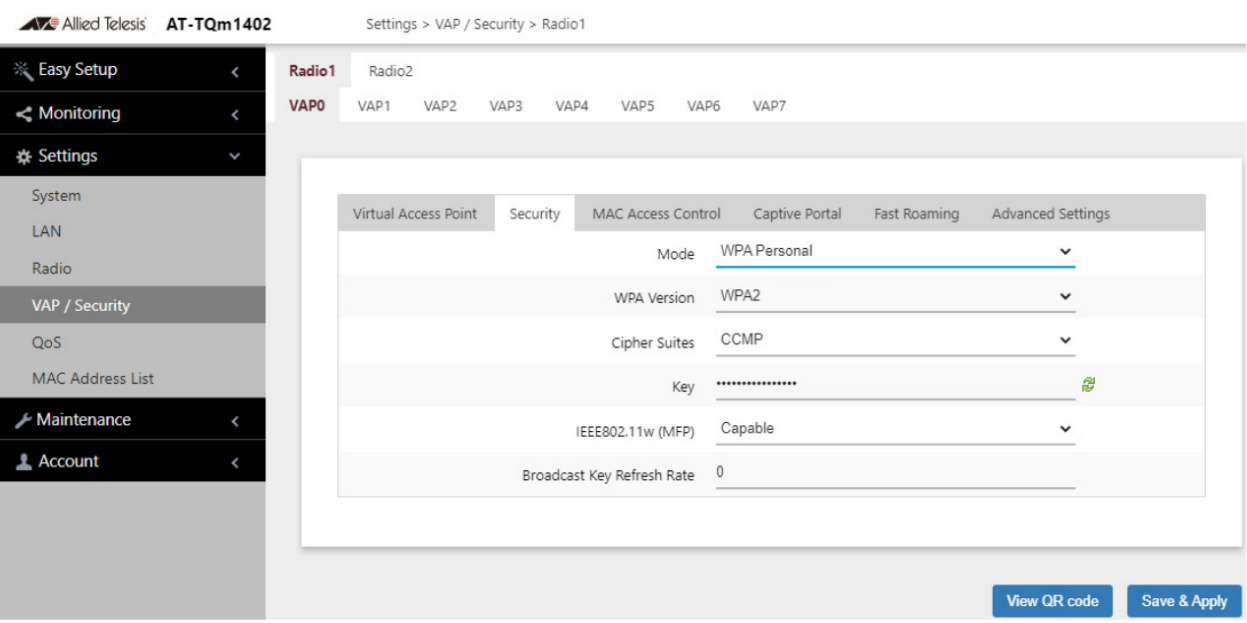
\includegraphics[width=0.9\textwidth]{images/point3}\\
        Рисунок 3.4.3 – Пример настройки Radio1 VAP0 Security
    \end{center}
    \\

    6. На странице «Account > User» задать новое имя пользователя в поле «Administrator Name»,
    ввести текущий пароль в поле «Current Password» (по умолчанию «friend»),
    задать новый пароль в полях «New Password» и «Confirm New Password» (см. рисунок ниже).
    Выбор конкретного имени пользователя и пароля должно сделать лицо, ответственное за обслуживание сети.

    \\
    \begin{center}
        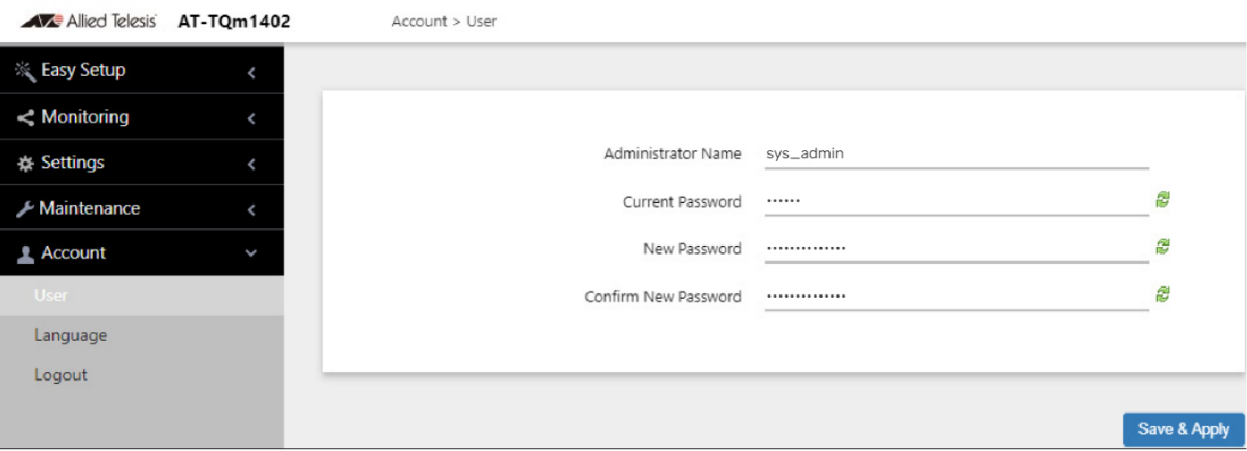
\includegraphics[width=0.9\textwidth]{images/point4}\\
        Рисунок 3.4.4 – Пример изменения данных для аутентификации
    \end{center}
    \\
    Аналогичные настройки производятся на второй точке беспроводного доступа.

    \subsubsection{Настройка IP-телефонов}
    Для начала следует настроить учетную запись MikoPBX.
    Перейдите в web-интерфейс MikoPBX.
    В разделе «Телефония» - «Сотрудники» добавьте новую запись для сотрудника.
    \\
    \begin{center}
        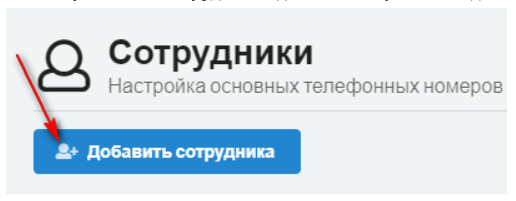
\includegraphics[width=0.5\textwidth]{images/users1}\\
        Рисунок 3.4.5 – Добавление новой записи для сотрудника
    \end{center}
    \\
    В разделе «Основные параметры»:
    «Номер» - внутренний номер телефона.
    «Пароль для SIP» - сложный пароль для SIP-учетной записи.
    Язык - Русский.
    \\
    \begin{center}
        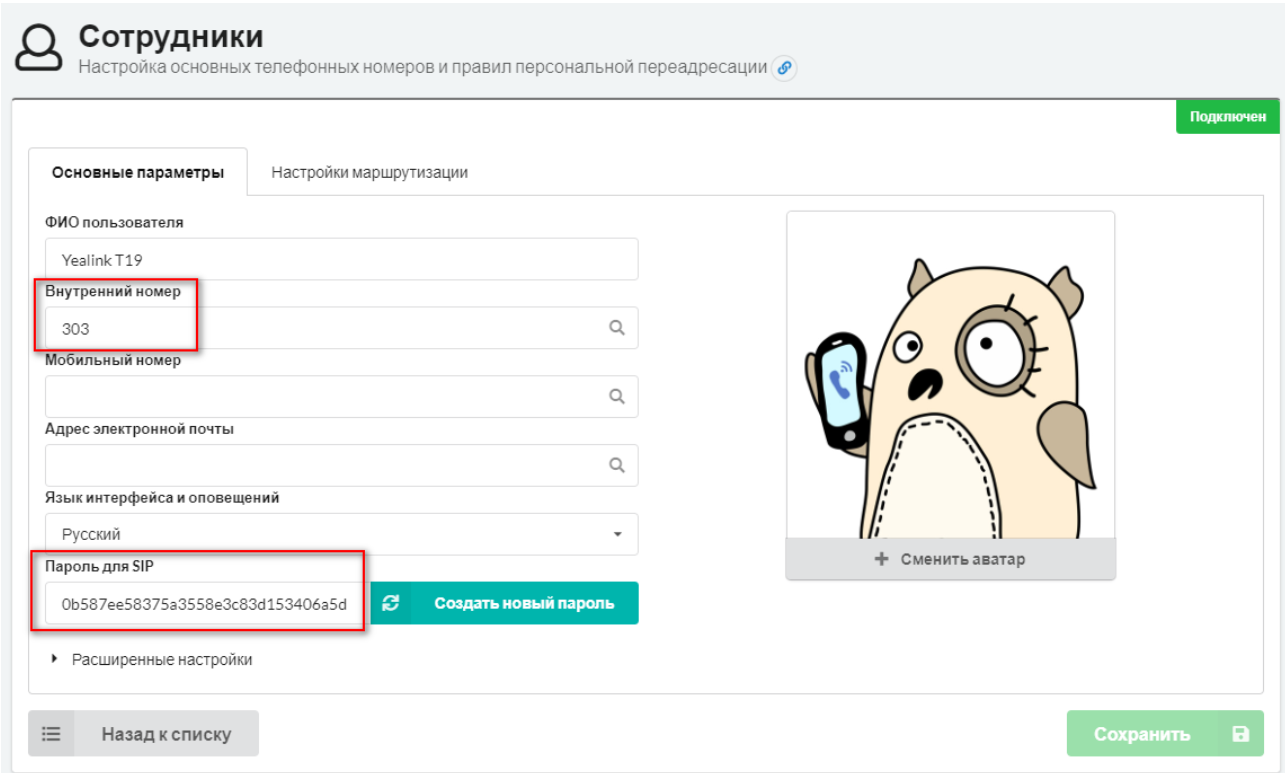
\includegraphics[width=0.8\textwidth]{images/main_config}\\
        Рисунок 3.4.6 – Задание параметров учетной записи
    \end{center}
    \\
    Сохраним изменения в учетной записи.
    Подключим телефон к сети через порт с надписью LAN.
    \\
    \begin{center}
        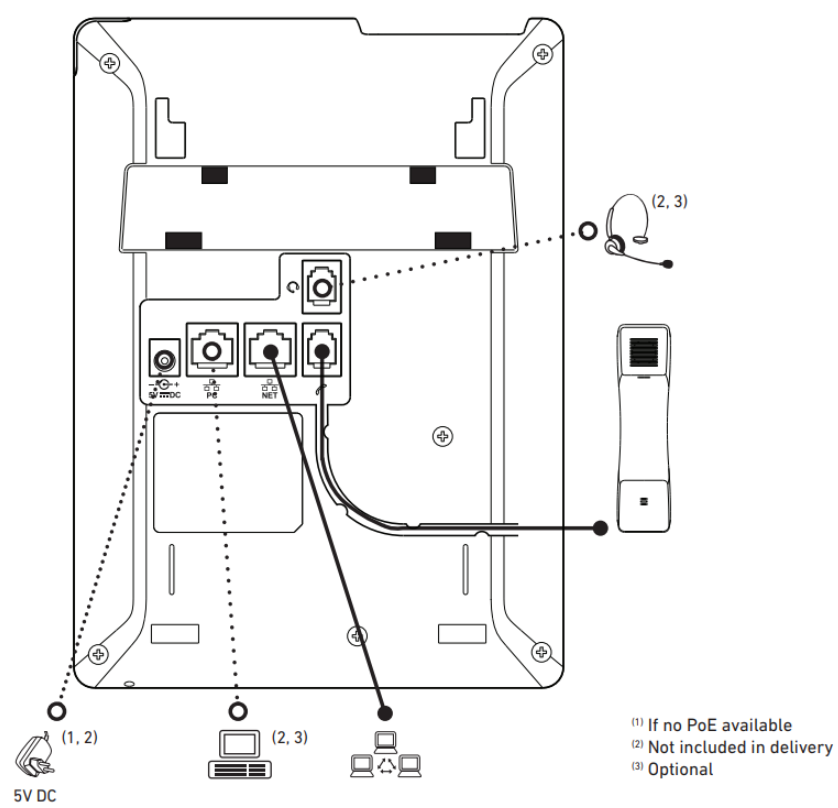
\includegraphics[width=0.8\textwidth]{images/phone_ports}\\
        Рисунок 3.4.7 – Расположение портов Snom D120
    \end{center}
    \\
    Так как у нас настроен DHCP, IP-телефон получит адрес автоматически.
    При включении адрес будет отображен на дисплее телефона.
    Перейдем в браузере по адресу IP-телефона, например http://79.108.212.170.
    Авторизуемся в web интерфейсе и для настройки учетной записи SIP перейдем в меню «Setup» - «Identity 1»,
    как показано на рисунке ниже:
    \\
    \begin{center}
        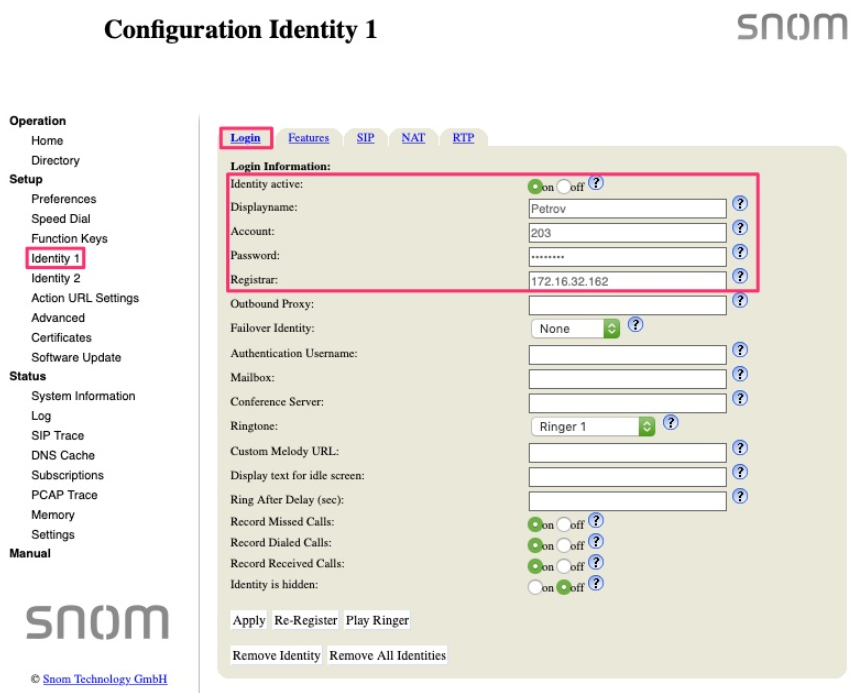
\includegraphics[width=0.8\textwidth]{images/identity1}\\
        Рисунок 3.4.8 – Настройка учетной записи SIP
    \end{center}
    \\

    Зададим следующие параметры:
    \begin{itemize}
        \item «Identity active» - установите в значение «on»
        \item «Displayname» - произвольное имя, лучше указать латиницей
        \item «Account» - идентификатор аккаунта - в MikoPBX совпадает с внутренним номером
        \item «Password» - пароль от учетной записи
        \item «Registrar» - адрес сервера MikoPBX
    \end{itemize}

    Нажмем кнопку «Apply» и выполним действие «Re-Register».
    Для проверки перейдём в раздел «Status» - «System Information».
    В случае успешной регистрации отобразится:
    \\
    \begin{center}
        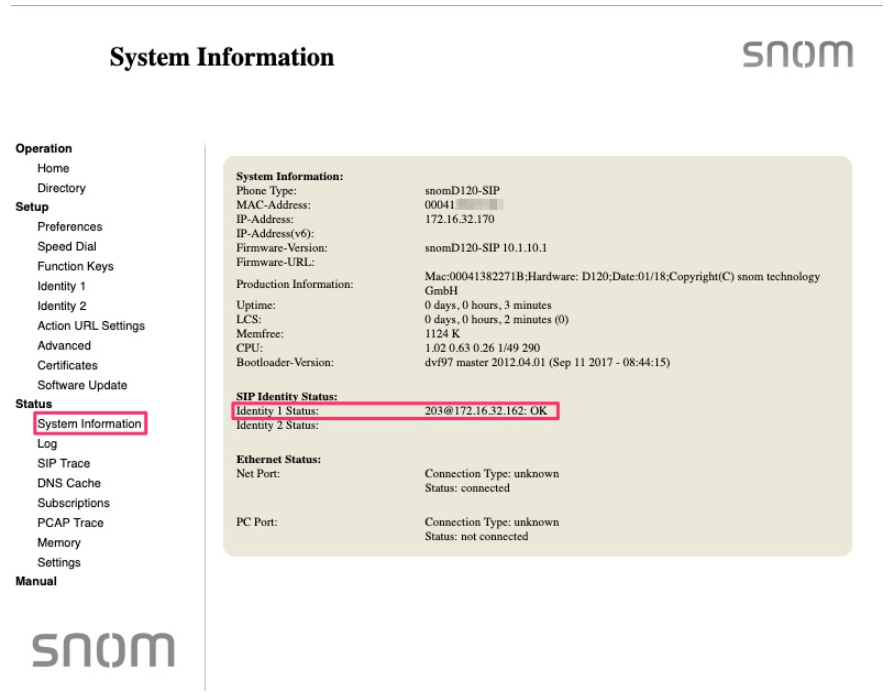
\includegraphics[width=0.8\textwidth]{images/check}\\
        Рисунок 3.4.9 – Проверка статуса настройки
    \end{center}
    \\

Также в Web-интерфейсе АТС, в списке сотрудников статус-иконка изменит цвет на зеленый:
    \\
    \begin{center}
        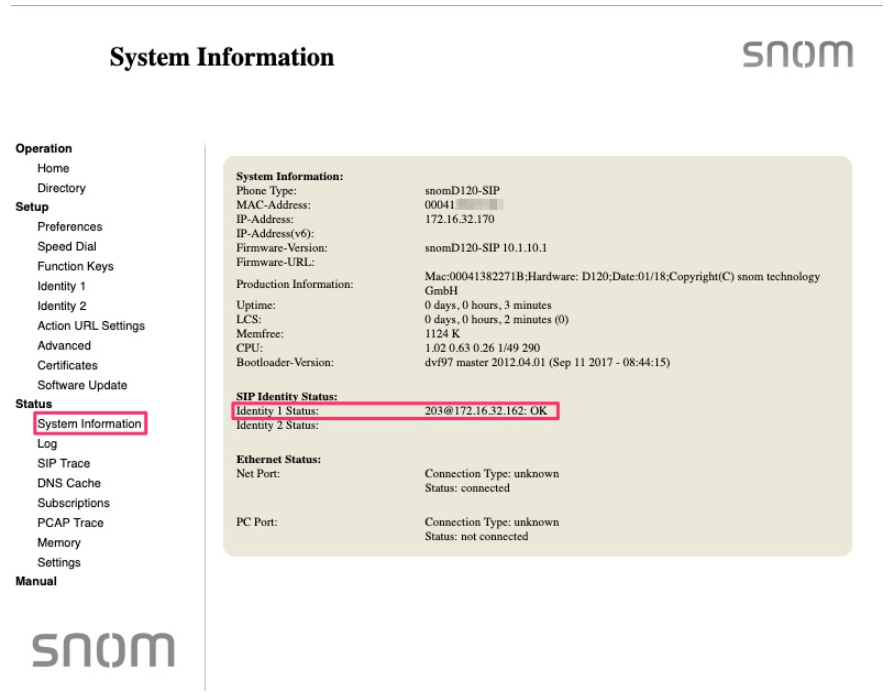
\includegraphics[width=0.8\textwidth]{images/check}\\
        Рисунок 3.4.10 – Проверка статуса настройки
    \end{center}
    \\

    Эти действия следует повторить для оставшихся IP-телефонов.

    \subsubsection{Настройка ПК}
    Так как персональные компьютеры получат свои адреса из DHCP диапозона,
    то их настройка ограничивается лишь установкой антивируса.
    Установка антивируса происходит через терминал.
    Для того чтобы открыть терминал в Linux Ubuntu нажимаем сочетание клавиш Alt + Ctrl + T.
    После этого вводим следующие команды:
\begin{lstlisting}
sudo apt-get update
sudo apt-get install clamav
\end{lstlisting}

    \subsubsection{Настройка принтера}
Принтер, как и персональные компьютеры получит свой адреса из DHCP диапозона,
поэтому его настройка ограничивается установкой драйвера.
Драйвер для принтера можно скачать на сайте производителя www.pantum.ru/support/download/driver.
Выберем и скачаем необходимый драйвер, как показано на рисунке ниже, однако поменяем операционную систему на Linux Ubuntu.

    \\
    \begin{center}
        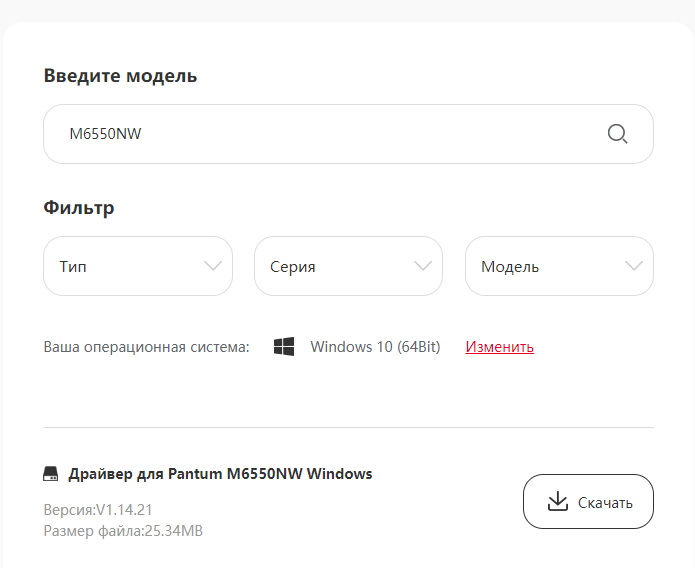
\includegraphics[width=0.8\textwidth]{images/printerdriver}\\
        Рисунок 3.4.11 – Скачивание драйверов принтера.
    \end{center}
    \\

Запустим драйвер на любом компьютере и следуем инструкции по установке.
После установки принтер должен быть доступен со всех компьютеров.

    \subsubsection{Настройка файлового сервера}
    Перед запуском файлового сервера необходимо установить жесткие диски.
    Для этого необходимо снять крышку, установить диск и закрепить шурупами как показано на рисунке 3.15.1.
    \\
    \begin{center}
        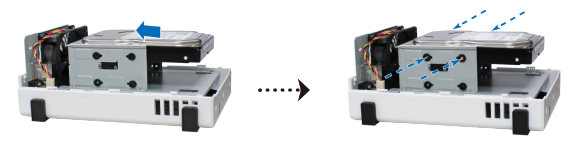
\includegraphics[width=0.8\textwidth]{images/disk}\\
        Рисунок 3.4.12 – Установка жесткого диска
    \end{center}
    \\
    Далее необходимо подключить сервер с помощью блока бесперебойного питания к сети, а также подключить его к коммутатору.
    Первым делом на любом из ПК зайдем в браузер и введем в браузере “find.synology.com”.
    Появится окно как на рисунке ниже:
    \\
    \begin{center}
        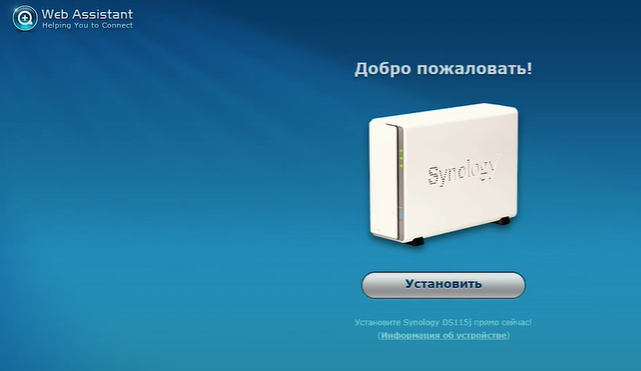
\includegraphics[width=0.8\textwidth]{images/OSDisk}\\
        Рисунок 3.4.13 – Окно установки операционной системы
    \end{center}
    \\
    Необходимо нажать кнопку установить, затем принять лицензионное соглашение и дождаться установки.
    После этого будет предложено задать имя сервера и создать учетную запись администратора – рисунок 3.15.3.
    Введем название “DISKSTATION”, имя admin и пароль.
    \\
    \begin{center}
        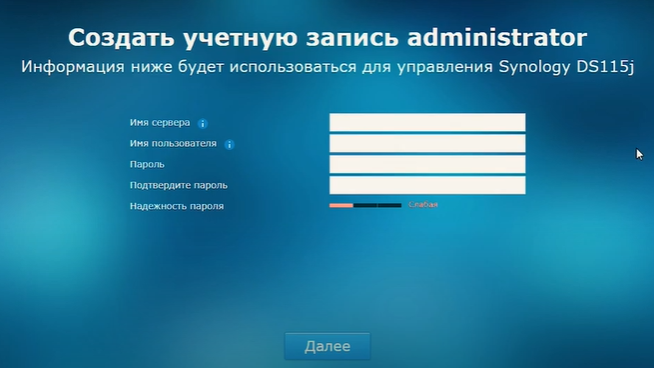
\includegraphics[width=0.8\textwidth]{images/login}\\
        Рисунок 3.4.15 – Создание учетной записи
    \end{center}
    \\
    Далее необходимо выбрать часовой пояс.

    Теперь перейдём в "Панель управления > Файловые службы > Настройки SMB",
    и установим флажок "Включить службу SMB", после нажмём "Применить".

    Далее настроим рабочую группу для реализации прав доступа, как показано на рисунке ниже.
    Имя рабочей группы может содержать от 1 до 15 символов.
    Имя не может содержать следующие символы: [ ] ; : " < > * + = \ / | ? ,
    Откроем "Панель управления > Пользователь и группа > Группа".
    Нажмем "Создать".
    Это действие запускает мастера создания группы.
    Введите имя и описание группы.
    Нажмите "Далее.
    Выполним оставшиеся шаги мастера, чтобы завершить создание группы.
    Нажмите "Применить", чтобы завершить.

    \\
    \begin{center}
        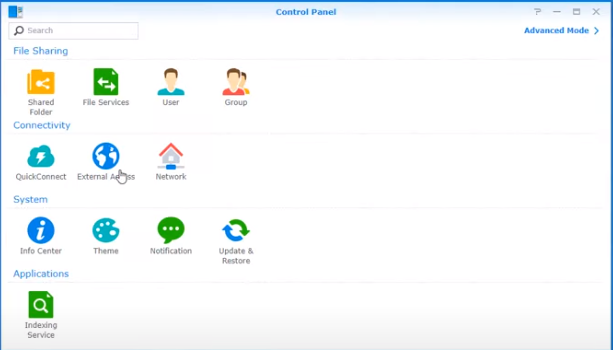
\includegraphics[width=0.8\textwidth]{images/creategroup}\\
        Рисунок 3.4.16 – Создание группы пользователей
    \end{center}
    \\

    Установим флажок "Скрыть общие папки от пользователей без разрешений",
    для того, чтобы пользователи не могли просматривать общие папки, для которых у них нет разрешений.

    После настроек, описанных выше пользователи будут отображены,
    как показано на рисунке ниже:

    \\
    \begin{center}
        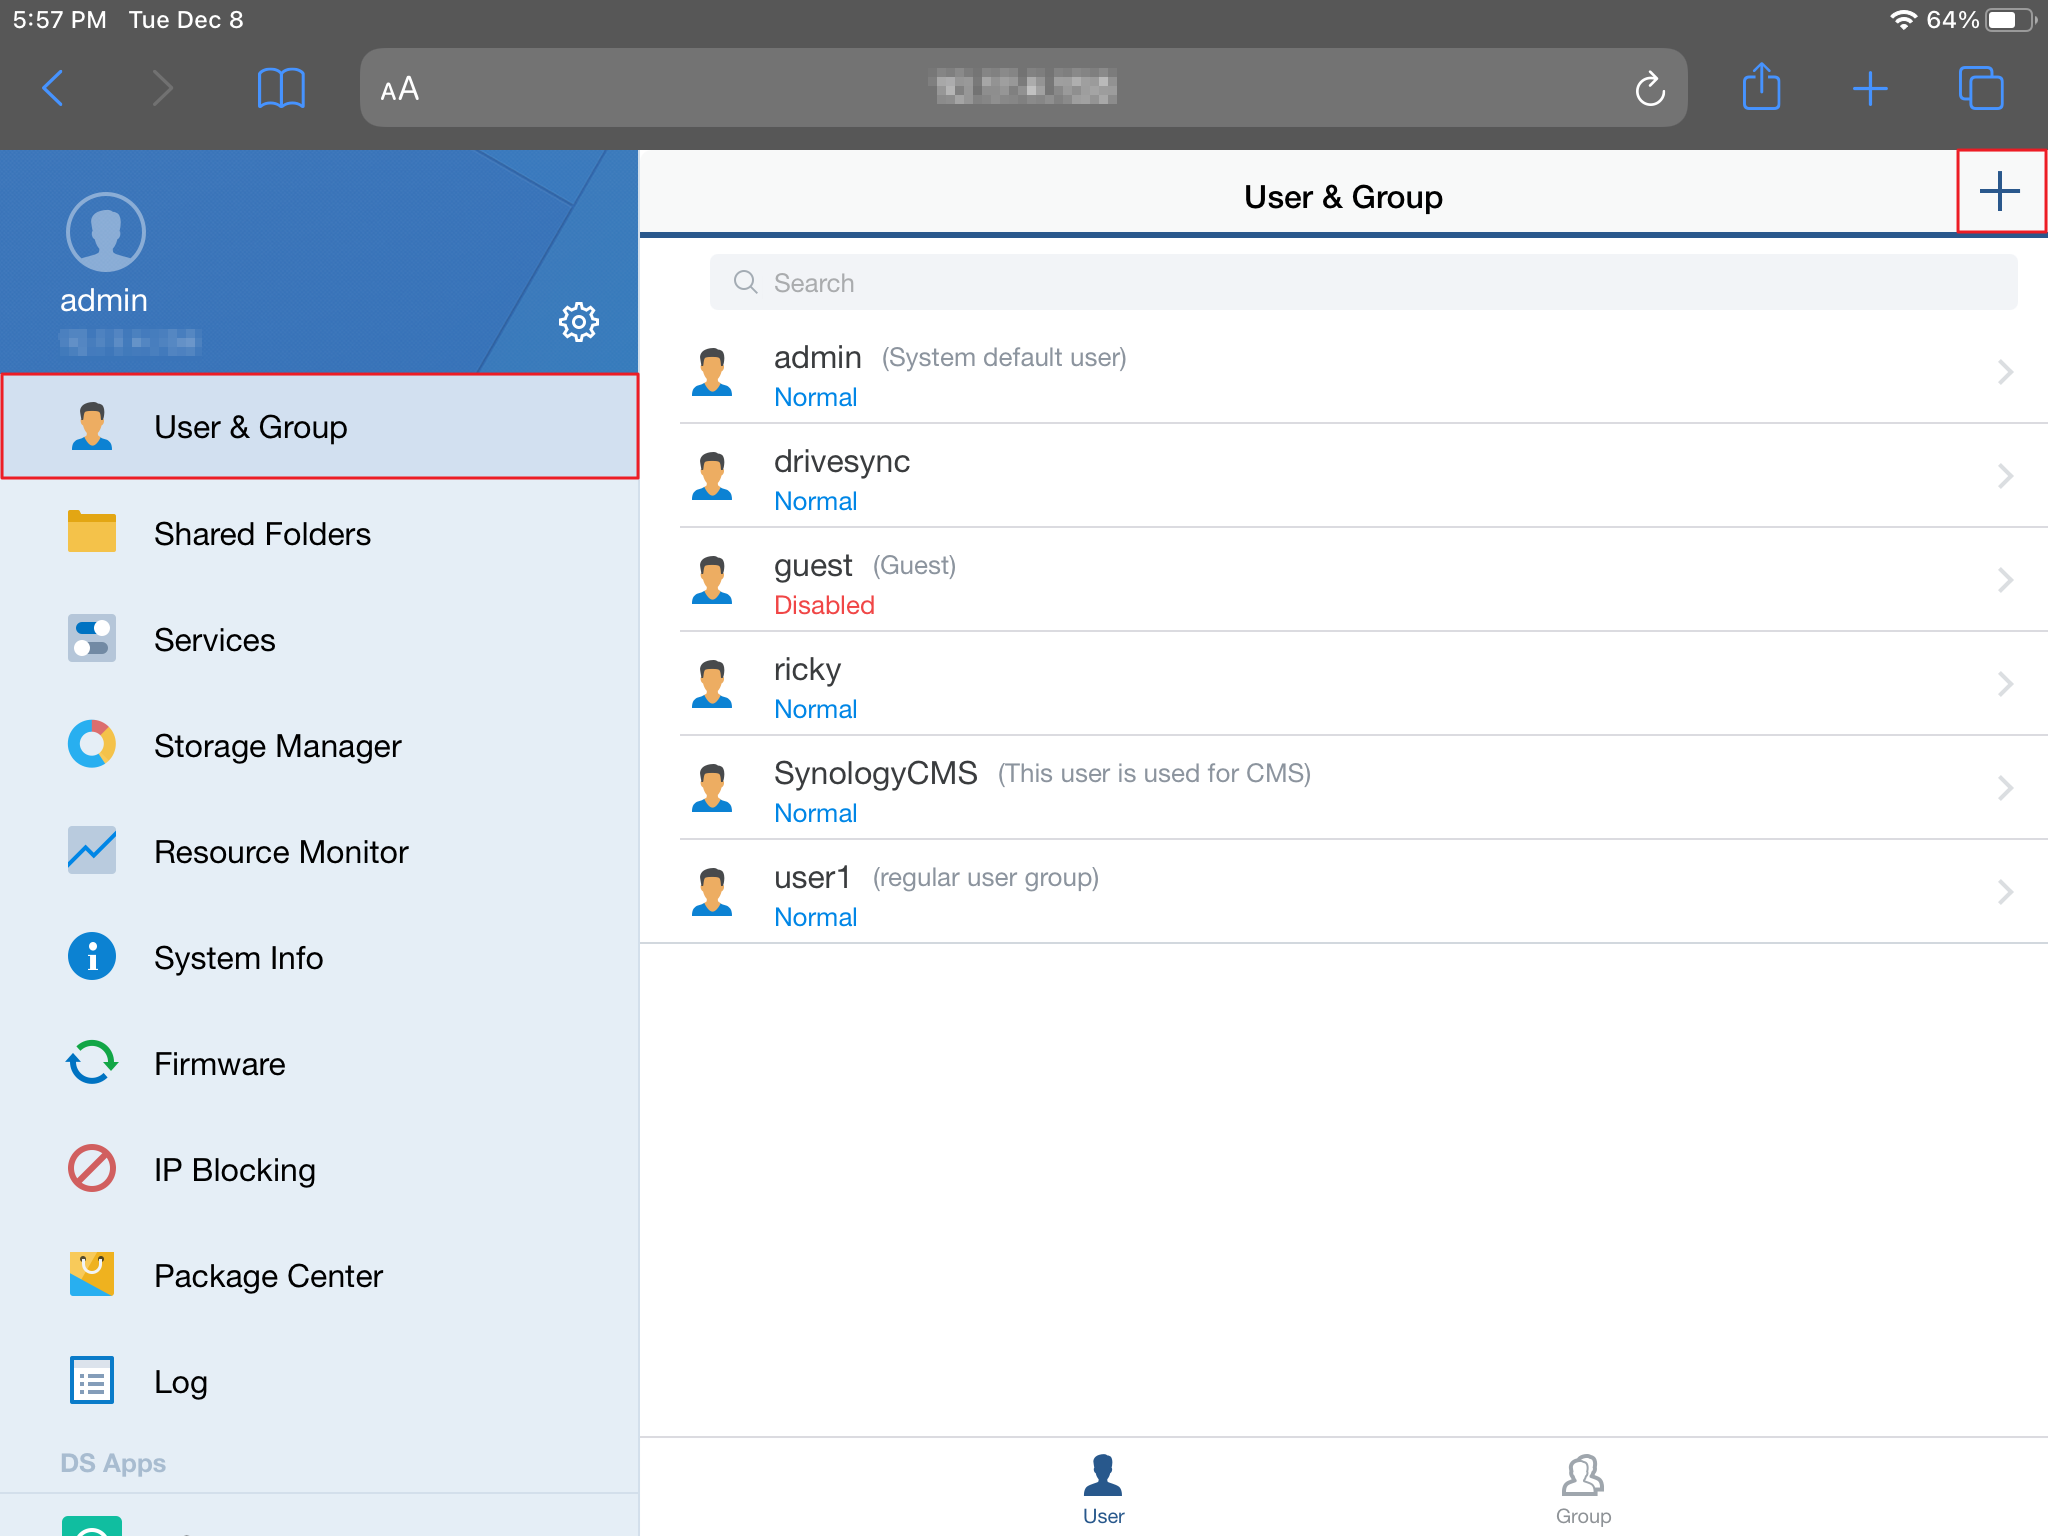
\includegraphics[width=0.8\textwidth]{images/usergroups}\\
        Рисунок 3.4.17 – Группы пользователей
    \end{center}
    \\


%\subsection{Выбор операционной системы}
%1. Простота установки и использования:
%   - Ubuntu славится своей дружественной к пользователю установкой и использованием.
%Установка проходит относительно легко, и для новичков в мире Linux, это может быть хорошим вариантом.
%
%2. **Обширное сообщество поддержки:**
%   - Ubuntu имеет большое и активное сообщество пользователей и разработчиков.
%Это обеспечивает обширный объем документации, форумов поддержки и ресурсов, где можно получить помощь.
%
%3. **Многообразие программного обеспечения:**
%   - Ubuntu поставляется с обширным набором предустановленного программного обеспечения,
%и также обеспечивает доступ к огромному количеству пакетов через свою систему управления пакетами APT.
%
%4. **Легкость в поиске и установке программ:**
%   - Система управления пакетами APT делает установку и обновление программного обеспечения относительно простым и безопасным процессом.
%
%5. **Snap-пакеты и Flatpak:**
%   - Ubuntu активно поддерживает технологии упакованных приложений Snap и Flatpak, облегчающих установку и обновление приложений.
%
%6. **LTS-версии:**
%   - Регулярно выпускаемые LTS-версии (с долгосрочной поддержкой) обеспечивают стабильность и обновления в течение долгого времени, что может быть важно для серверных и корпоративных сред.
%
%7. **Поддержка аппаратного обеспечения:**
%   - Ubuntu имеет широкую поддержку аппаратного обеспечения, что делает его хорошим выбором для использования на различных устройствах.
%
%Эти плюсы делают Ubuntu хорошим выбором для многих пользователей, особенно для тех, кто только начинает использовать Linux или ищет дистрибутив с хорошей общественной поддержкой и обширной базой программного обеспечения. Однако, конечный выбор всегда зависит от конкретных потребностей и предпочтений пользователя.


%\subsection{Выбор модели рабочей станции}
% Based on https://tex.stackexchange.com/a/352349/139966
%\begin{table}[ht]
%    \caption{Рабочие станции}
%    \label{table:func:workStantionsProperty}
%    \begin{tabular}{| >{\raggedright}m{0.310\textwidth}
%                    | >{\raggedright\arraybackslash}m{0.310\textwidth}
%                    | >{\raggedright\arraybackslash}m{0.310\textwidth}|}
%        \hline
%        \centering Название & \centering\arraybackslash Комплектующие & \centering\arraybackslash Средняя оценка/количество отзывов \\
%
%        \hline
%        HP 200 G4 1C7L8ES &
%        21.5" 1920 x 1080 IPS, матовый, несенсорный, Intel Core i5 10210U 4200 МГц, 8 ГБ, SSD 256 ГБ, видеокарта встроенная, LAN 1 Gbit, WiFi 802.11ac &
%        5/1
%        \\
%        \hline
%        MSI Pro AP242 12M-209XRU &
%        23.8" 1920 x 1080 IPS, матовый, несенсорный, Intel Core i3 12100 4300 МГц, 8 ГБ, SSD 512 ГБ, видеокарта встроенная, LAN 1 Gbit, WiFi 802.11ax &
%        5/1
%        \\
%        \hline
%        Lenovo IdeaCentre 3 24ITL6 F0G0017ELK &
%        23.8" 1920 x 1080 IPS, матовый, несенсорный, Intel Core i5 1135G7 4200 МГц, 8 ГБ, HDD 1000 ГБ, видеокарта встроенная, LAN 1 Gbit, WiFi 802.11ax &
%        3.5/3
%        \\
%
%        \hline
%    \end{tabular}
%\end{table}


%\subsection{Выбор модели принтера}
%Принтер в НИО АСУ играет важную роль во всех отделах,
%обеспечивая печать документов, отчетов, графиков, схем, технической документации и других материалов.
%Для принтера следует выделить следующие требования:
%
%\begin{itemize}
%    \item Качество печати и размер;
%    \item Большой объем печати;
%    \item Совместимость и подключение;
%    \item Экономичность;
%\end{itemize}
%
%
%Совместимость и подключение определяется типами интерфейсов для подключения, совместимость драйверов с операционными
%системами (далее OC), а также сетевыми возможностями.
%Рассмотрим в таблице 2.2 данные аспекты.
%
%\begin{table}[ht]
%    \caption{Совместимость и подключение}
%    \label{table:func:printersConnectionProperty}
%    \begin{tabular}{| >{\raggedright}m{0.475\textwidth}
%                    | >{\raggedright\arraybackslash}m{0.475\textwidth}|}
%        \hline
%        \centering Аспекты подключения и совместимости & \centering\arraybackslash Описание \\
%
%        \hline
%        Типы интерфейсов для подключения &
%        USB, Ethernet, Wi-Fi, Bluetooth.
%        \\
%        \hline
%        Совместимость драйверов с ОС &
%        Windows, Linux, MacOS
%        \\
%        \hline
%        Сетевые возможности &
%        Поддержка проводных и беспроводных сетей
%        \\
%
%        \hline
%    \end{tabular}
%\end{table}
%
%
%Для выбора существующих принтеров также воспользуемся сайтом-агрегатором Onliner.by.
%Для этого следует определиться с характеристиками принтера в соответствии с требованиями приведенными выше.
%
%\begin{table}[ht]
%    \caption{Модели принтеров}
%    \label{table:func:printersList}
%    \begin{tabular}{| >{\raggedright}m{0.225\textwidth}
%                    | >{\raggedright\arraybackslash}m{0.225\textwidth}
%                    | >{\raggedright\arraybackslash}m{0.225\textwidth}
%                    | >{\raggedright\arraybackslash}m{0.225\textwidth}|}
%        \hline
%        \centering Модель
%        & \centering\arraybackslash Качество печати/размер
%        & \centering\arraybackslash Совместимость
%        & \centering\arraybackslash Подключения \\
%
%        \hline
%        h & h & h & h
%        \\
%
%        \hline
%    \end{tabular}
%\end{table}

%......................


%\subsection{Выбор файлового сервера}

%\subsection{Выбор модели точки доступа}



%\subsection{Выбор модели IP-телефонов}




%\subsection{Выбор модели коммутатора}\label{subsec:func:switchChoice}
%\begin{table}[ht]
%    \caption{Характеристики производителя}
%    \label{table:func:manufacturerList:1}
%    \begin{tabular}{| >{\raggedright}m{0.100\textwidth}
%                    | >{\raggedright\arraybackslash}m{0.190\textwidth}
%                    | >{\raggedright\arraybackslash}m{0.190\textwidth}
%                    | >{\raggedright\arraybackslash}m{0.190\textwidth}
%                    | >{\raggedright\arraybackslash}m{0.190\textwidth}|}
%        \hline
%        \centering Модель
%        & \centering\arraybackslash Присутствие на рынке
%        & \centering\arraybackslash Поддержка
%        & \centering\arraybackslash Инновации
%        & \centering\arraybackslash Доступность \\
%
%        \hline
%        Cisco &
%        Широкий спектр высококачественного сетевого оборудования. Является лидером на рынке. &
%        Имеет услуги поддержки, предлагает обучающие программы и курсы &
%        Постоянно внедряет новые технологии и стандарты &
%        Дорогостоящее оборудование
%        \\
%        \hline
%        HPE &
%        Предлагает обширную линейку как сетевого оборудования так и других технологических решений. Популярен на рынке
%        оборудования коммерческого уровня &
%        Хорошая поддержка, которая отвечает различным потребностям бизнеса &
%        Внедряет облачные технологии  и технологии программно-определяемых сетей (software-defined networks) &
%        Конкурентная цена оправданная предлагаемыми возможностями.
%        \\
%        \hline
%    \end{tabular}
%\end{table}
%\begin{table}[ht]
%    \caption{Характеристики производителя}
%    \label{table:func:switchsList}
%    \begin{tabular}{| >{\raggedright}m{0.100\textwidth}
%                    | >{\raggedright\arraybackslash}m{0.200\textwidth}
%                    | >{\raggedright\arraybackslash}m{0.250\textwidth}
%                    | >{\raggedright\arraybackslash}m{0.100\textwidth}
%                    | >{\raggedright\arraybackslash}m{0.200\textwidth}|}
%        \hline
%        \centering Модель
%        & \centering\arraybackslash Кол-во портов
%        & \centering\arraybackslash Поддержка Gigabit портов
%        & \centering\arraybackslash Комм. способность
%        & \centering\arraybackslash Безопасность \\
%
%        \hline
%        Catalyst 9300X &
%        12-24 (multi-rate 1/2.5/5/10/25G SFP28), 24-48 (1/2.5/5/10G Multigigabit) &
%        100G, 40G, 25G, 10G, 1G fiber &
%        1-2 Тбит/с &
%        AES-256/MACsec-256, SSH, TLS, IPsec, IGMP snooping, MPLS, NetFlow, Аналитика зашифрованного трафика
%        \\
%
%        \hline
%        Catalyst 9300LM &
%        24-48 &
%        40G, 25G, 10G, 1G fiber Multigigabit, 10G/5G/2.5G/1G, 10/100/1000BASE-T copper &
%        56-472 Гбит/с &
%        AES-256/MACsec-256, SSH, TLS, IPsec, IGMP snooping, MPLS, NetFlow, Аналитика зашифрованного трафика
%        \\
%
%        \hline
%        Catalyst 9300 &
%        24-48 &
%        40G, 25G, 10G, 1G fiber, Multigigabit, 10G/5G/2.5G/1G, 10/100/1000BASE-T copper &
%        208-640 Гбит/с &
%        AES-256/MACsec-256, SSH, TLS, IPsec, IGMP snooping, MPLS, NetFlow, Аналитика зашифрованного трафика
%        \\
%
%        \hline
%        Catalyst 9300L &
%        24-48 &
%        40G, 25G, 10G, 1G fiber Multigigabit, 10G/5G/2.5G/1G, 10/100/1000BASE-T copper &
%        56-472 Гбит/с &
%        AES-256/MACsec-256, SSH, TLS, IPsec, IGMP snooping, MPLS, NetFlow, Аналитика зашифрованного трафика
%        \\
%        \hline
%    \end{tabular}
%\end{table}

%\subsection{Выбор маршрутизатора}\label{subsec:func:router}

%\subsection{Выбор пассивного сетевого оборудования}

%\subsubsection{Выбор сетевого шкафа}
%
%\subsubsection{Выбор кабеля}
%
%Так как в требованиях заказчика есть пункт "повышенная пожарная безопасность",
%то выбор кабеля ограничевается параметром
%
%\subsubsection{Выбор коннектора, короба и розетки}
%
%В характеристиках кабеля указан лишь диаметр проводника – 24AWG, поэтому для расчета размера короба возьмем максимальный диаметр кабеля как 6мм.
%В большинстве мест нам нужно проложить либо 2, либо 6 кабелей, поэтому возьмем короба размерами 25x16 идущие от и между шкафов и 15x10 идущие непосредственно к розеткам.
%Возьмем следующие короба:
%\begin{itemize}
%    \item Leiden ELECTRIC 15x10;
%    \item Leiden ELECTRIC 25x16.
%\end{itemize} \\
%
%Также возьмем коннекторы “ЮПИТЕР RJ-45 8P8C” и розетки “PST00 39047”.
%
%\subsection{Конфигурация сетевого оборудования}
%
%По заданию выдана подсеть 25.237.242.0/23.
%Сеть будет разделена на 5 подсетей.
%Назначение и адреса подсетей указаны в таблице 3.9.1.
%
%\begin{table}[ht]
%    \caption{Схема адресации подсетей}
%    \label{table:func:vlans}
%    \begin{tabular}{| >{\raggedright}m{0.250\textwidth}
%                    | >{\raggedright\arraybackslash}m{0.100\textwidth}
%                    | >{\raggedright\arraybackslash}m{0.300\textwidth}
%                    | >{\raggedright\arraybackslash}m{0.200\textwidth}|}
%        \hline
%        \centering Назначение
%        & \centering\arraybackslash VLAN
%        & \centering\arraybackslash Адрес подсети
%        & \centering\arraybackslash Маска подсети \\
%
%        \hline
%        Административная & 4 & 192.168.4.0 & 255.255.255.0 \\
%        \\
%
%        \hline
%        Внутренние устройства & 7 & FD9B:8283:105B:665D::/64 \\
%        \\
%
%        \hline
%        Стационарные ПК & 7 & 25.237.242.160 & 255.255.255.224 \\
%        \\
%
%        \hline
%        Внутренняя беспроводная & 8 & 25.237.242.128 & 255.255.255.224 \\
%        \\
%
%        \hline
%
%        Гостевая беспроводная & 10 & 25.237.242.32 & 255.255.255.240 \\
%        \hline
%    \end{tabular}
%\end{table}
%
%Публичные IPv4 адреса будут использоваться на всех устройствах, имеющих доступ в интернет.
%Частные IPv4 адреса использованы в административной подсети, в которую будет включено такое оборудование, как маршрутизатор, коммутаторы и точки доступа.
%Всем ПК, серверу и принтерам будут присвоены unique local адреса для общения внутри сети.
%Адреса в административной подсети указаны в таблице 3.9.2.
%
%%\begin{table}
%%    \centering
%%    \begin{tabular}{ll}
%%        \toprule
%%        \textbf{Устройство} & \textbf{Адрес} \\
%%        \midrule
%%
%%        Маршрутизатор & 192.168.4.1 \\
%%
%%        Точка доступа (1 этаж) & 192.168.4.12 \\
%%
%%        Точка доступа (2 этаж) & 192.168.4.22 \\
%%
%%        Точка доступа (3 этаж) & 192.168.4.32 \\
%%        \bottomrule
%%    \end{tabular}
%%    \caption{Адресация административной подсети}
%%    \label{tab:admin}
%%\end{table}
%
%
%\subsubsection{Настройка маршрутизатора}
%Для начала нужно подключиться к CLI маршрутизатора.
%С помощью кабеля идущего в комплекте подключить маршрутизатор к компьютеру через консольный порт.
%Расположение порта указано на рисунке как Console port.
%
%\centering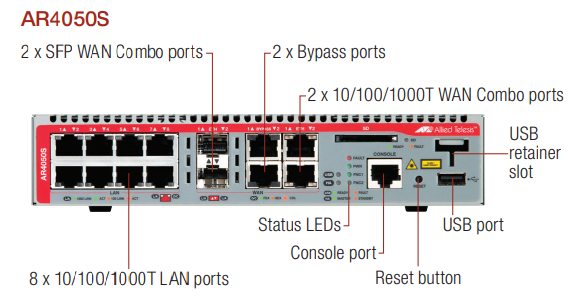
\includegraphics[width=0.5\textwidth]{images/router_config}\label{image:func:routersPorts}
%\centering Рисунок 228 – Расположение портов на AR4050
%
%Далее с помощью любого клиентского приложения, поддерживающего работу через последовательный порт, например PuTTY начнем работу с маршрутизатором.
%При настройке других сетевых устройств, в частности точек доступа будем по возможности использовать протокол AMF, который позволяет обнаружить и настроить устройства в сети.
%Сразу после подключения включим маршрутизатор, зададим имена ему и сети и сделаем его мастером в сети:
%\begin{verbatim}
%    Awplus>enable
%    Awplus#conf terminal
%    Awplus(config)#hostname Router
%    Router(config)#atmf network-name company
%    Router(config)#atmf master
%\end{verbatim}
%
%Также создадим агрегированный канал через который будет проходить соединение с коммутатором на 3 этаже.
%\begin{verbatim}
%    Router(config)#interface port1.0.0
%    Router(config-if)#channel-group 2 mode active
%    Router(config-if)#exit
%    Router(config)#interface port1.0.1
%    Router(config-if)#channel-group 2 mode active
%    Router(config-if)#exit
%\end{verbatim}
%
%Дальнейшие настройки будут производиться через интерфейс с названием “po2”.
%Занесем в сеть коммутатор подключенный через данный интерфейс:
%\begin{verbatim}
%Router(config)#interface po2
%Router(config-if)#switchport atmf-link
%\end{verbatim}
%
%Далее создадим VLAN-ы.
%Создание административного VLAN-а:
%\begin{verbatim}
%    Router (config)#vlan database
%    Router (config-vlan)#vlan 4 name vlan4 enable
%    Router (config-vlan)#exit
%    Router (config)#int vlan4
%    Router (config-if)#ip address 192.168.4.0/24
%\end{verbatim}
%
%Настроим маршрутизацию между сетями.
%Для этого для настроим подинтерфейсы для каждого VLAN-а из таблицы 3.9.1. На примере административного VLAN-а пропишем команды:
%\begin{verbatim}
%    Router (config)#int po2.4
%    Router (config-if)# encapsulation dot1q 4
%    Router (config-if)# ip address 192.168.4.1/24
%\end{verbatim}
%
%Далее настроим RIP. Добавим все подсети:
%\begin{verbatim}
%    Router (config)#router rip
%    Router (config-router)# network 25.237.242.32/28
%    Router (config-router)# network 25.237.160.32/27
%    Router (config-router)# network 25.237.128.32/27
%\end{verbatim}
%
%\subsubsection{Настройка коммутаторов}
%\subsubsection{Настройка DHCP сервера}
%\subsubsection{Настройка стационарных компьютеров}
%
%\subsubsection{Настройка беспроводных точек доступа}
%
%\subsubsection{Настройка файлового сервера}
%
%
%\subsubsection{Настройка принтера}
%
%\subsubsection{Настройка IP-телефона}
